\documentclass{beamer}

\usepackage[spanish, mexico]{babel}
\usepackage[utf8]{inputenc}
\usepackage{csvsimple}
\usepackage{listingsutf8}
\usepackage{longtable}
\usepackage{subcaption}
\usepackage{graphicx}
\usepackage{float}

\usetheme{Frankfurt}
\graphicspath{{../figuras/}}
\author{Federico Soto Badilla, Diego Osvaldo Ochoa de la Cruz}
\title{Osciloscopio con Arduino}
\date{30 de mayo del 2018}
\titlegraphic{
\includegraphics[height=1.5cm]{uabc.png}\hfill
\includegraphics[height=1.5cm]{fcs.jpg}}

\newcommand{\tab}{\indent\indent}
%\renewcommand{\theenumi}{\alph{enumi})}

\begin{document}
\maketitle

\section{Objetivos}
\begin{frame}
\frametitle{Objetivos}
\begin{itemize}
\item Aprender a utilizar la tarjeta Arduino.
\item Aprender a graficar en tiempo real en Python.
\item Utilizar lo aprendido en clase para poder elaborar un osciloscopio.
\end{itemize}
\end{frame}

\section{Funcionamiento}
\begin{frame}
\frametitle{Funcionamiento}
\framesubtitle{Lista de materiales}
\noindent
\textbf{Electrónicos}
\begin{itemize}
\item Arduino UNO
\item Computadora
\item 8 Resistencias de 1kOhm
\end{itemize}
\textbf{Mecánico}
\begin{itemize}
\item Protoboard
\item Jumpers
\end{itemize}
\textbf{Software}
\begin{itemize}
\item Editor de Arduino
\item Python
\end{itemize}
\end{frame}

\begin{frame}
\frametitle{Funcionamiento}
\framesubtitle{Circuito}
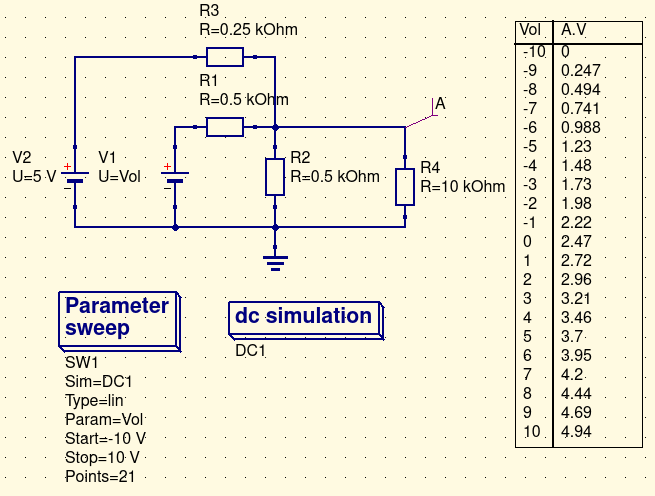
\includegraphics[width=0.9\textwidth]{CirSim.png}
\end{frame}

\begin{frame}
\frametitle{Funcionamiento}
\framesubtitle{Programa}
\centering
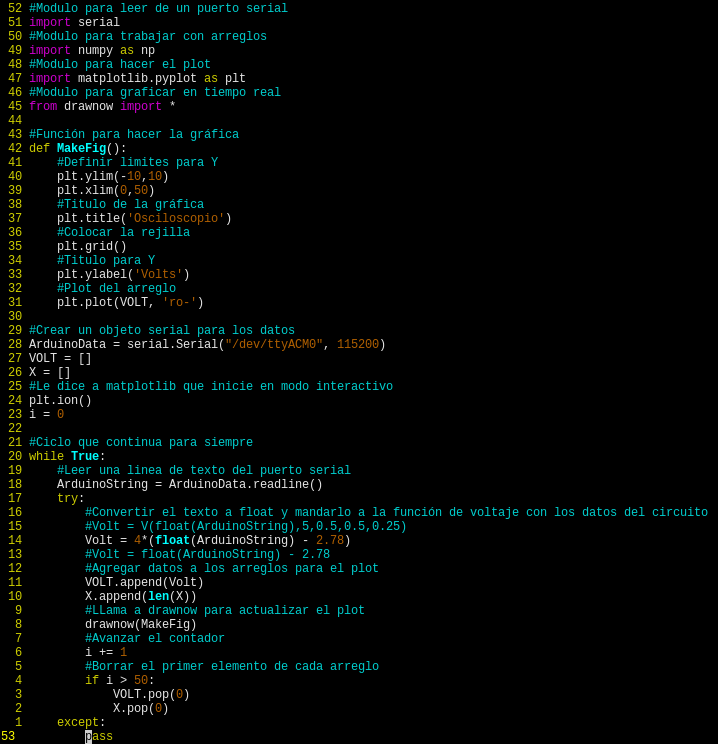
\includegraphics[height=0.8\textheight]{CodPy.png}
\end{frame}

\section{Resultados}
\begin{frame}
\frametitle{Resultados}
\centering
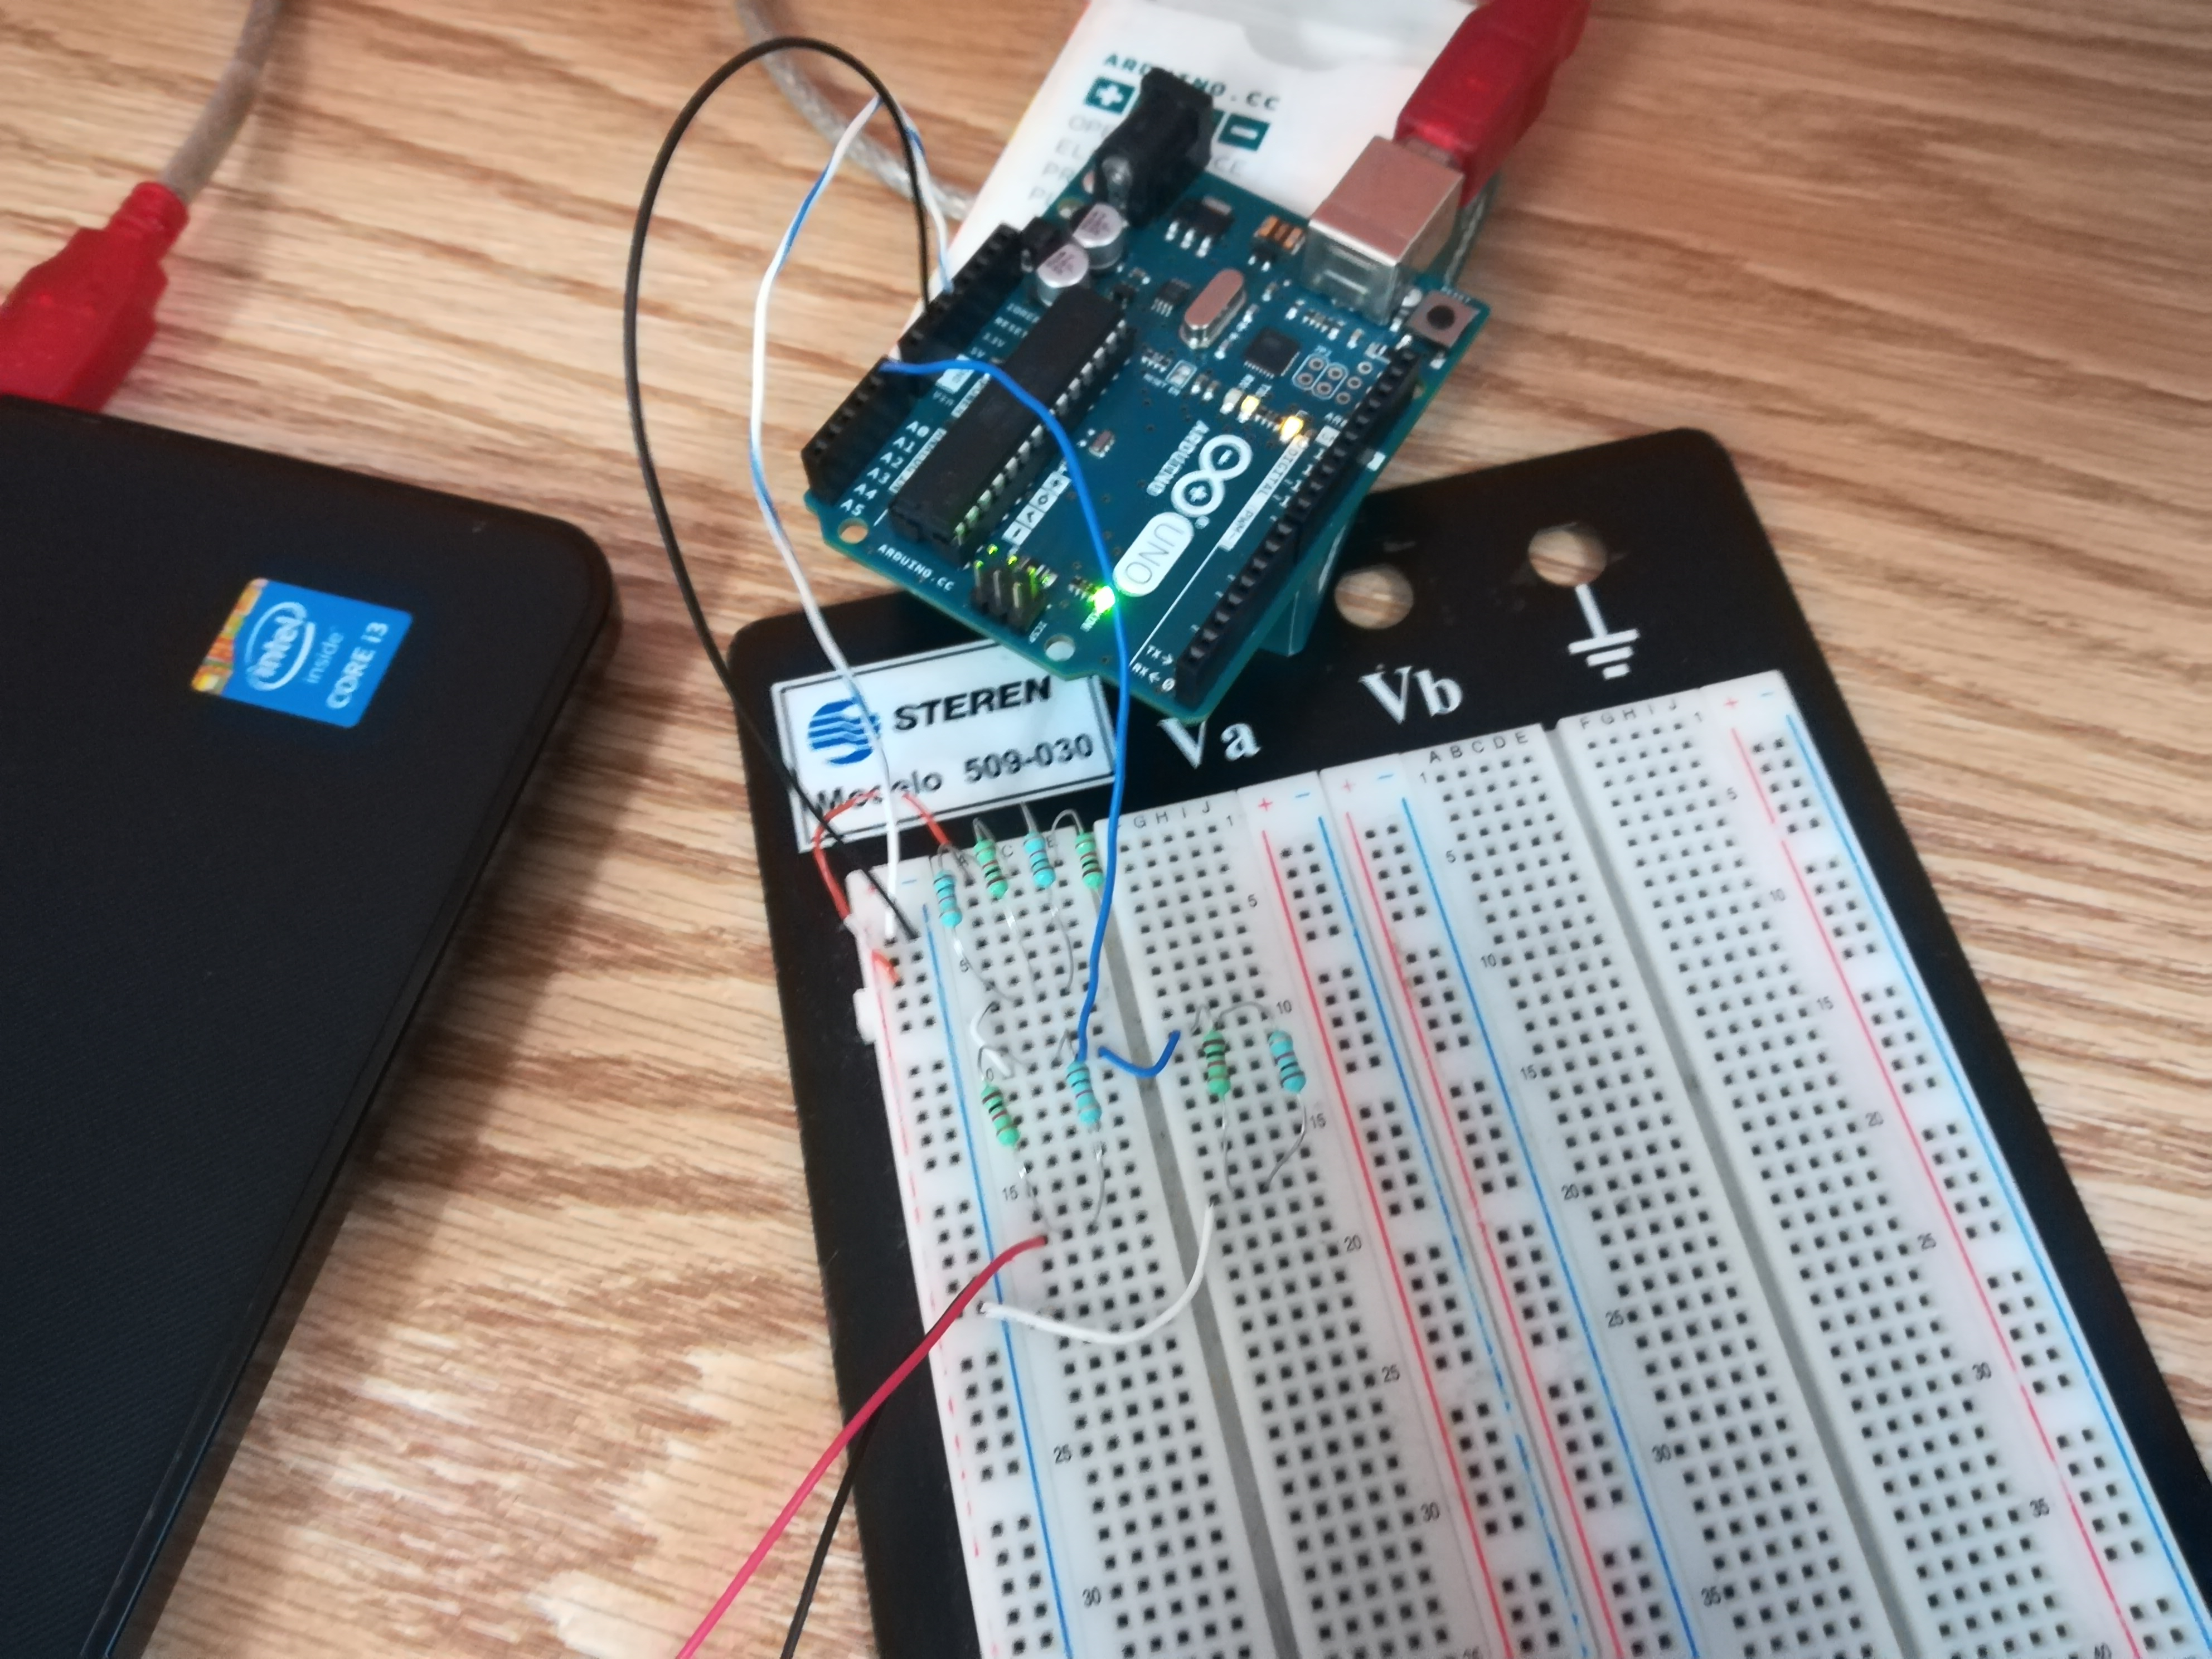
\includegraphics[width=0.45\textwidth]{Cir1.jpg}
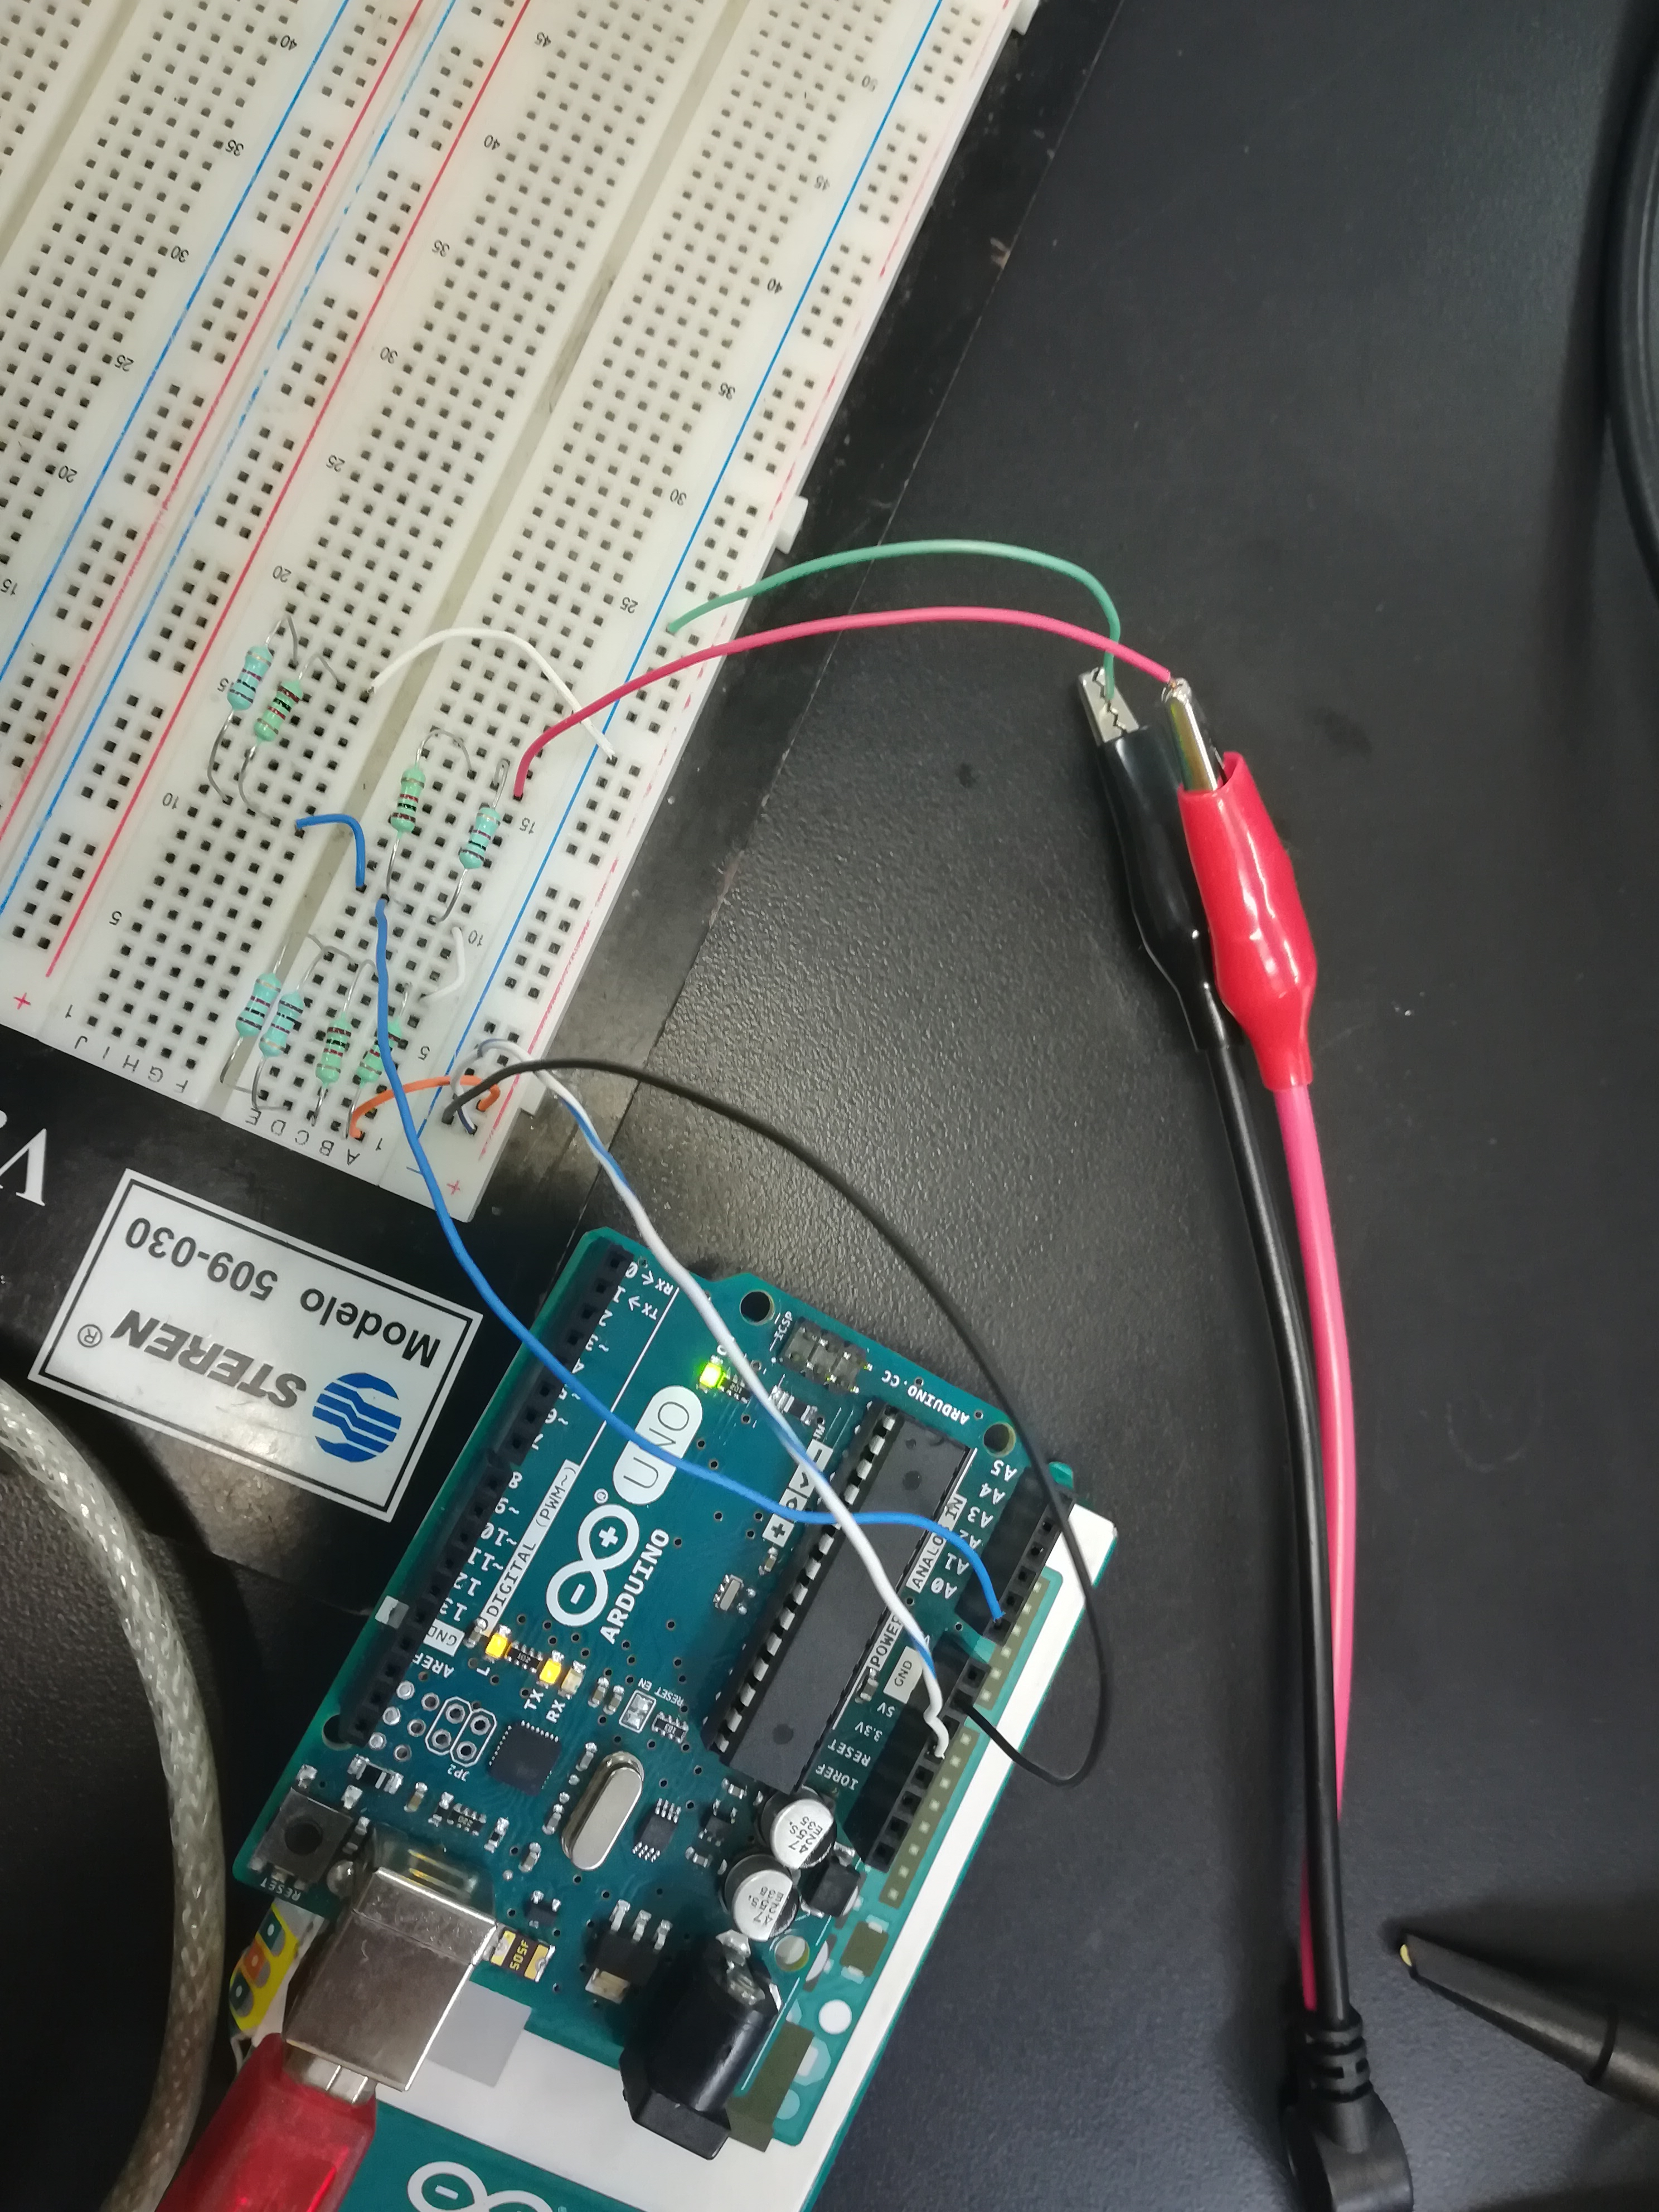
\includegraphics[width=0.45\textwidth]{Cir2.jpg}
\end{frame}

\begin{frame}
\frametitle{Resultados}
\centering
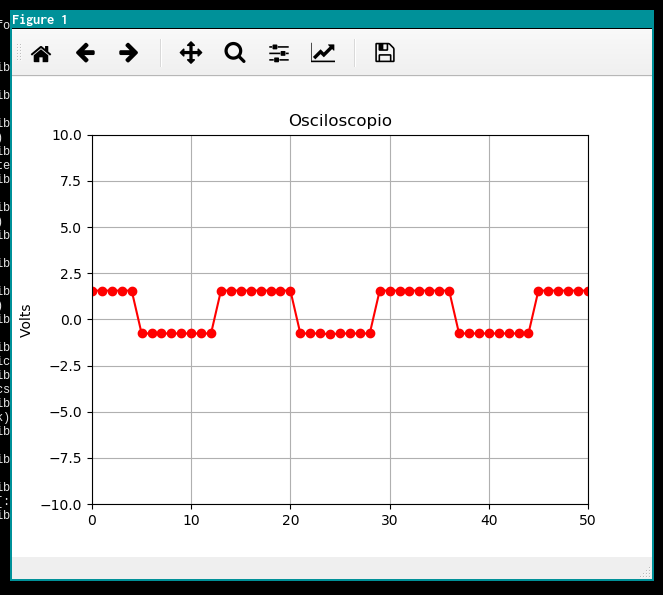
\includegraphics[width=0.45\textwidth]{Osc1.png}
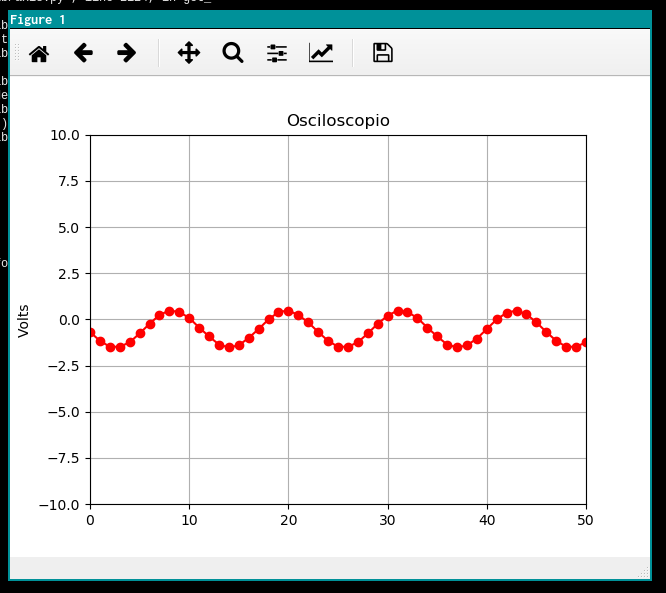
\includegraphics[width=0.45\textwidth]{Osc2.png}
\end{frame}
\end{document}
